\documentclass[10pt, conference]{IEEEtran}
\IEEEoverridecommandlockouts
% The preceding line is only needed to identify funding in the first footnote. If that is unneeded, please comment it out.
\usepackage{cite}
\usepackage{booktabs}
\usepackage{amsmath,amssymb,amsfonts}
\usepackage{algorithmic}
\usepackage{graphicx}
\usepackage{threeparttable}
\usepackage{textcomp}
\usepackage{xcolor}
\def\BibTeX{{\rm B\kern-.05em{\sc i\kern-.025em b}\kern-.08em
    T\kern-.1667em\lower.7ex\hbox{E}\kern-.125emX}}
\begin{document}

\title{ManyTypes4Py: A benchmark dataset for machine learning-based type inference\\
%{\footnotesize \textsuperscript{*}Note: Sub-titles are not captured in Xplore and
%should not be used}
%\thanks{Identify applicable funding agency here. If none, delete this.}
}

\author{\IEEEauthorblockN{Amir M. Mir}
\IEEEauthorblockA{\textit{Department of Software Technology} \\
\textit{Delft University of Technology}\\
Delft, The Netherlands \\
s.a.m.mir@tudelft.nl}
\and
\IEEEauthorblockN{Evaldas Latoškinas}
\IEEEauthorblockA{\textit{Department of Software Technology} \\
\textit{Delft University of Technology}\\
Delft, The Netherlands \\
e.latoskinas@student.tudelft.nl}
\and
\IEEEauthorblockN{Georgios Gousios}
\IEEEauthorblockA{\textit{Department of Software Technology} \\
\textit{Delft University of Technology}\\
Delft, The Netherlands \\
g.gousios@tudelft.nl}
}

\maketitle

\begin{abstract}

\end{abstract}

\begin{IEEEkeywords}
\end{IEEEkeywords}

\section{Introduction}
Dynamic programming languages (DPLs) give developers fast prototyping as they do not require static types at compile-time. However, lack of static typing causes several issues such as unexpected run-time exceptions, sub-optimal support for integrated development environments (IDEs), and less precise program analysis. To address these issues, optional static typing is introduced for DPLs like Python \cite{van2014pep}, JavaScript \cite{bierman2014understanding}, PHP \cite{klingstrom2020type}. Yet, developers are required to manaually add type annotations to their existing codebases, which is a labarious task \cite{ore2018assessing}.

In recent years, machine learning (ML) techniques has been successfully applied to tackle problems in sofware engineering (SE) \cite{allamanis2018survey}, including but not limited to, type inference \cite{allamanis2020typilus, pradel2019typewriter}, code completion \cite{svyatkovskiy2019pythia}, code changes \cite{tufano2019learning}, and bug detection \cite{qiao2020deep}. This research area is often called \textit{ML4SE}, which is new and emerging.

ML techniques need a large and high-quality dataset to achieve an acceptable level of generalization for the task at hand \cite{sun2017revisiting}. In the ML community, there are quite a number of well-known visual and text datasets \cite{pouyanfar2018survey}. For the SE problems, several research efforts have been made to create datasets to facilitate further research with data-driven models. For instance, Karampatsis et al. \cite{karampatsis2020often} recently published the ManySStuBs4J dataset for repairing simple bugs in Java programs. 

Concerning the ML-based type inferece for DPLs, it is difficult to create a benchmark dataset that contains a sufficient number of software projects with type annotations. Because of the optional static typing, many software projects written in DPLs lack type annotations. Nevertheless, to train an ML-based type inference model, researchers ended up creating their own dataset by either gathering a small set of projects with type annotations \cite{pradel2019typewriter} or employ static type inference tools to add type annotations to existing projects \cite{allamanis2020typilus}, which makes the learning task weak.



\begin{figure*}[!t]
	\centering
	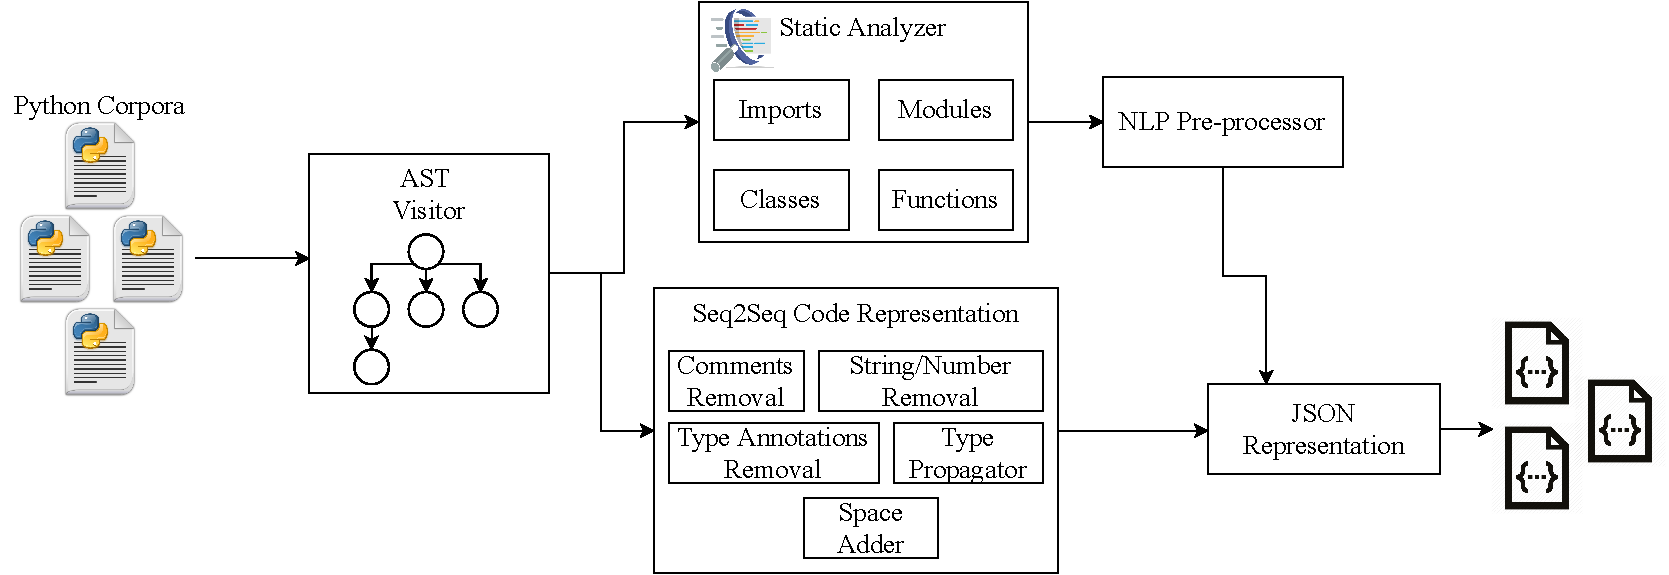
\includegraphics[width=\linewidth]{figs/manytypes4py-pipeline.pdf}
	\caption{Overview of light-weight static analysis pipeline}
	\label{fig:overview-pipeline-sa}
\end{figure*}

\section{Methodology}
We created ManyType4Py dataset using the following methodology:

\begin{itemize}
	\item To find Python projects with type annotations, we intuitively search for projects that has mypy as a depdendency on libraries.io. Since mypy is the most used type checker for Python, projects that use mypy have most likely type annotations. Our search resulted in 5,382 Python projects that are publicly available on GitHub. We cloned all the discovered projects on the disk in Sep. 2020 and finally created a file that contains projects' URL and their latest commit hash. The resulting dataset is roughly 60 GB in size before pre-processing.
	\item As demonstrated by Allamanis \cite{allamanis2019adverse}, it is essential to de-duplicate a code corpora. Because code duplication negatively affects the performance of machine learning models when testing on duplicated code corpora. Following this, we de-duplicated the collected Python corpora in the previous step using our code de-duplication tool, namely, CD4Py\footnote{https://github.com/saltudelft/CD4Py}. In short, the CD4Py tool tokenizes Python source code files, vectorizes files using term frequency-inverse document (TF-IDF), and performs $k$-nearest neighbor search to identify candidate duplicates files. Out of 636,383 Python source code files, 354,409 files were identified as duplicate and they are removed from the code corpora.
	\item After the removal of duplicate files, we split the Python code corpora into three sets by files, i.e., 70\% training data, 10\% validation data, and 20\% test data. This is a common practice that is considered in recent research work \cite{pradel2019typewriter, allamanis2020typilus}, concerning machine learning-based models for type inference.
	% file extensions removal might worth mentioning here
	\item Given the de-duplicated code corpora and a list of files for the three sets, we ran our light-weight static analysis pipeline, which is depicted in Figure \ref{fig:overview-pipeline-sa}. First, the Abstract Syntax Tree (AST) of Python source files are extracted and nodes in ASTs are visited. Second, using the light-weight static analyzer, type-related information are extracted from imports, modules, classes, and functions. Third, the seq2seq representation of source code files \cite{hellendoorn2018deep} are generated by removing comments, string, number literals, and propagating types. Forth, common NLP practices such as tokenization and lemmatization are applied to idenfier names in source code files. Finally, the processed Python projects are stored as a JSON-formatted file which is described in Table \ref{tab:json-fields}. 
\end{itemize}

After completing all the aforementioned steps, a zip file is created which contains: (1) JSON file of processed projects (2) a file containing projects' URL and their latest commit hash (3) a file containing duplicate files in the dataset (4) a CSV file containing a list of files and their corresponding set. The ManyTypes4Py dataset together with its helper scripts and instructions are publicly available on GitHub\footnote{https://github.com/saltudelft/many-types-4-py-dataset}.

\section{Description}

\begin{table*}[t]
	\centering
	\caption{Description of fields in the JSON file of projects produced by the pipeline}
	\label{tab:json-fields}
	\begin{tabular}{c l}
		\toprule
		Field Name in the JSON & Description \\
		\midrule
		\multicolumn{2}{c}{Project}  \\
		\midrule
		\texttt{author/repo} & The name of a project and its author on the GitHub URL  \\
		\midrule
		\texttt{src\_files} & Contains the path of a project's source code files \\
		\midrule
		\texttt{file\_path} & The path of a source code file to differentiate it with other files \\
		\midrule
		\multicolumn{2}{c}{Module}  \\
		\midrule
		\texttt{untyped\_seq} & The normalized seq2seq representation of a source code file \\
		\midrule
		\texttt{typed\_seq} & Contains the type of identifiers in \texttt{untyped\_seq} if present. Otherwise $0$ is inserted. \\
		\midrule
		\texttt{imports} & Contains the name of imports in a source code file. \\
		\midrule
		\texttt{variables} & Contains variables' name and their type defined in a module (i.e. global variables) \\
		\midrule
		\texttt{classes} & Contains the JSON object of processed classes in a module which is described below \\
		\midrule
		\texttt{funcs} &  Contains the JSON object of processed functions in a module, which are described below \\
		\midrule
		\texttt{set} & The set to which a source code file belongs to, i.e., \texttt{train}, \texttt{valid}, \texttt{test} \\
		\midrule
		\multicolumn{2}{c}{Class} \\
		\midrule
		\texttt{name} & The name of a processed class in a module \\
		\midrule
		\texttt{variables} & Contains class variables' name and their type if present \\
		\midrule
		\texttt{funcs} & Contains the JSON object of processed functions in a class, which are described below \\
		\midrule
		\multicolumn{2}{c}{Function} \\
		\midrule
		\texttt{name} & The name of a processed function in either a class or a module \\
		\midrule
		\texttt{params} & Contains a processed function's parameter names and their type if present \\
		\midrule
		\texttt{ret\_exprs} & Contains the return expression(s) of a processed function \\
		\midrule
		\texttt{ret\_type} & The return type of a processed function if present \\
		\midrule
		\texttt{variables} & Contains local variables' name and their type in a function \\
		\midrule
		\texttt{params\_occur} & Contains parameters and their usages in the body of a processed function \\
		\midrule
		\texttt{docstring} & Contains docsting of a processed function if present, which has the below subfields \\
		\midrule
		\texttt{docstring.func} & One-line description of a processed function \\
		\midrule
		\texttt{docstring.ret} & Description of what a processed function returns \\
		\midrule
		\texttt{docstring.long\_descr} & Long description of a processed function \\
		\bottomrule
	\end{tabular}
\end{table*}

\begin{table}
	\centering
	\caption{Duplication statistics across the ManyTypes4Py dataset}
	\begin{tabular}{c c}
		\toprule
		Duplication stats & Value \\
		\midrule
		\# Detected duplicate files & 400,245 (78.43\%) \\
		\# Detected clusters & 45,836 \\
		Avg. \# of files per clusters & 8.73 \\
		Median \# of files per clones & 3.00 \\
		Duplication ratio & 69.45\% \\
		\bottomrule
	\end{tabular}
\end{table}

\begin{table}
\centering
\caption{Characteristics of the ManyTypes4Py Dataset}
\begin{threeparttable}
\begin{tabular}{l c}
	\toprule
	Metrics & Value \\
	\midrule
	Repositories & 5,382 \\
	Files & 183,916 \\
	Lines of code\tnote{a} & 22M \\
	\midrule
	Functions & 2,096,797 \\
	...with comment & 1,129,573 (53.8\%) \\
	...with return type annotations & 325,532 (15.5\%)  \\
	\midrule
	Arguments & 3,923,667 \\
	...with comment & 220,976 (5.6\%) \\ 
	...with type annotations & 480,793 (12.2\%) \\
	\midrule
	Types & 869,825 \\
	...unique & 67,060 \\
	\bottomrule
\end{tabular}
	\begin{tablenotes}
	\item[a] {\footnotesize Comments and blank lines are ignored when counting lines of code.}
\end{tablenotes}
\end{threeparttable}
\end{table}


\begin{figure}[!t]
	\centering
	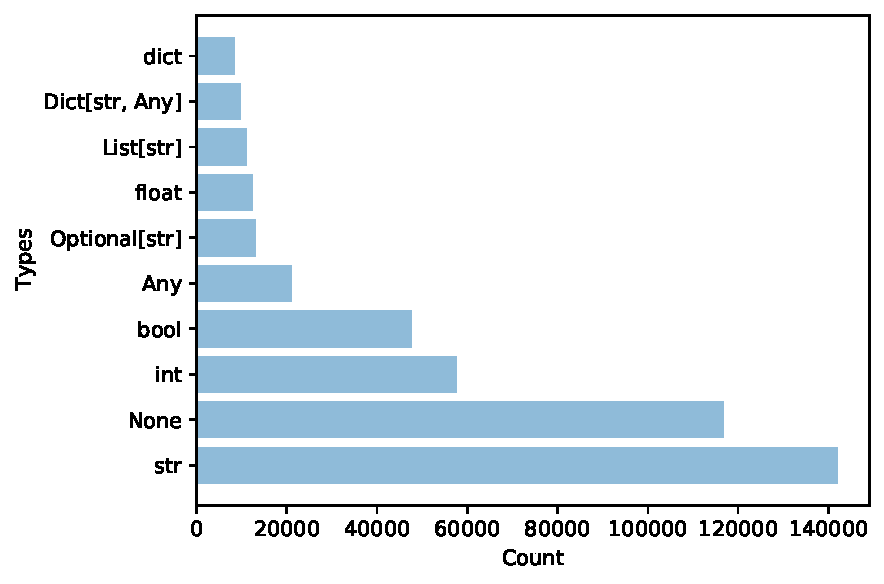
\includegraphics[width=\linewidth]{figs/top-10-most-frequent-types.pdf}
	\caption{Top 10 most frequent types in the ManyTypes4Py dataset}
	\label{fig:top-10-types}
\end{figure}

\section{Applications}
% Type inference 

% Code compeletion

\section{Benchmark}

\section{Related Work}
There are several Python code corpora that can be used for machine learning-based type inference. Recently, Allamanis et al. \cite{allamanis2020typilus} proposed the Typilus model, which is a graph-based neural model that predicts type annotations for Python. The Typilus model \cite{allamanis2020typilus} accompanies with a relatively small dataset that contains 600 Python projects. Moreover, the source code files of Typilus' dataset are converted to graph representations that are only suitable for training the Typilus model. However, the ManyTypes4Py dataset provides JSON-formatted analyzed source code files that contains useful type hints for training various machine learning models. Raychev et al. \cite{raychev2016probabilistic} published the Python-150K dataset in 2016, which contains 8,422 Python projects. Unlike our dataset, the Python-150K dataset \cite{raychev2016probabilistic} is not collected for the ML-based type inference task, meaning that a large of number projects in the dataset may not have type annotations at all. Moreover, Allamanis \cite{allamanis2019adverse} showed that the Python-150K suffers from duplication despite the removal of project forks.


\section{Conclusion}

\section*{Acknowledgment}

\bibliographystyle{IEEEtran}
\bibliography{main}

\end{document}
